\documentclass{beamer}
\beamertemplatenavigationsymbolsempty
\usepackage[french]{babel}
\usepackage{fontspec}
\usepackage{amsmath, amsthm, amsfonts}
\usepackage[separate-uncertainty]{siunitx}
\usepackage{xcolor}
\usepackage{tikz}
\usepackage{tikz-cd}
\usepackage[object=vectorian]{pgfornament}
\usepackage{circuitikz}
\usepackage{hyperref}
\usepackage{caption}
\usepackage{booktabs}
\usepackage{mathtools}
\usepackage{longtable}
\usepackage[version=3]{mhchem}
\usepackage{marginnote}
\usepackage[framemethod=tikz]{mdframed}


% Paul Tol's qualitative palette
% ``bright''.https://personal.sron.nl/~pault/#sec:qualitative
\definecolor{tblue}{HTML}{4477AA}
\definecolor{tcyan}{HTML}{66CCEE}
\definecolor{tgreen}{HTML}{228833}
\definecolor{tyellow}{HTML}{CCBB44}
\definecolor{tred}{HTML}{EE6677}
\definecolor{tpurple}{HTML}{AA3377}
\definecolor{tgrey}{HTML}{BBBBBB}


% Justification for marginnotes.
\renewcommand*{\raggedleftmarginnote}{}
\renewcommand*{\raggedrightmarginnote}{}


% Styles for mdframed environments.
\newmdenv[backgroundcolor=tgreen!10,linecolor=tgreen!30]{reponsebox}
\newmdenv[backgroundcolor=tyellow!10,linecolor=tyellow!30]{diapobox}
\newmdenv[backgroundcolor=tred!10,linecolor=tred!30]{fondamentalbox}

% Default arrow for tikz and style for positive and negative objects.
\tikzset{>=latex,
    negative/.style={draw=teal!70!black, fill=teal!10, thick},
    positive/.style={draw=red, fill=red!10, thick}}
\usetikzlibrary{matrix,calc,decorations.pathreplacing,decorations.pathmorphing,decorations.markings}

% French locale for numbers and negative exponent for units.
\sisetup{locale=FR, per-mode=symbol}

\newcommand{\abs}[1]{\left| #1 \right|}
\newcommand{\rhat}{\vec{\hat{r}}}
\newcommand{\xhat}{\vec{\imath}}
\newcommand{\yhat}{\vec{\jmath}}
\newcommand{\zhat}{\vec{k}}
\newcommand{\real}{\mathbb{R}}
\newcommand{\der}[2]{\frac{\mathrm{d}#1}{\mathrm{d}#2}}
\newcommand{\pder}[2]{\frac{\partial\ #1}{\partial\ #2}}
\newcommand{\dif}{\mathrm{d}}
\newcommand{\ddif}{\,\mathrm{d}}
\newcommand{\grad}{\vec{\nabla}}
\newcommand{\exemple}[1]{\begin{fullwidth}#1\end{fullwidth}}
\newcommand{\norm}[1]{\lVert\ #1\ \rVert}
\newcommand{\vu}{\vec{u}}
\newcommand{\vv}{\vec{v}}
\newcommand{\vr}{\vec{r}}
\newcommand{\va}{\vec{a}}
\newcommand{\vF}{\vec{F}}
\newcommand{\vE}{\vec{E}}
\newcommand{\vB}{\vec{B}}
\newcommand{\vecxyz}[3]{#1 \xhat\ + #2 \yhat\ + #3 \zhat}
\newcommand{\vecxy}[2]{#1 \xhat\ + #2 \yhat}
\newcommand{\coulombcst}{k}
\newcommand{\emf}{\ensuremath{\mathcal{E}}}
\newcommand{\eval}{\SI{1.602e-19}{C}}
\newcommand{\kval}{\SI{8.99e9}{Nm^2 \per C^2}}

% Nice separator line
\newcommand{\sectionline}{
    \noindent
    \begin{center}
        \resizebox{0.5\linewidth}{1ex}
    {{%
    {\begin{tikzpicture}
    \node  (C) at (0,0) {};
    \node (D) at (9,0) {};
    \path (C) to [ornament=85] (D);
    \end{tikzpicture}}}}
    \end{center}
}

\theoremstyle{definition}
\newtheorem*{defn}{Definition}


\usepackage[version=3]{mhchem}

\definecolor{UniBlue}{RGB}{83,121,170}
\setbeamercolor{title}{fg=UniBlue}
\setbeamercolor{frametitle}{fg=UniBlue}
\setbeamercolor{structure}{fg=UniBlue}

\begin{document}

\begin{frame}{Champ électrique d'une charge ponctuelle}
  \begin{center}
  \begin{tikzpicture}[ampersand replacement=\&]
    \matrix[column sep=1.5cm] {
    \node[positive, circle] (q) at (0, 0) {$+$};
    \foreach \theta in {0, 30, ..., 330} {
      \draw[->] (q) -- ++(\theta:1);
      \draw[->] ($(q) + (\theta:1.05)$) -- ++(\theta:0.5);
      \draw[->] ($(q) + (\theta:1.05) + (\theta:0.55)$) -- ++(\theta:0.25);
    }
    \&
    \node[negative, circle] at (0, 0) {$-$};
    \foreach \theta in {0, 30, ..., 330} {
      \draw[<-] (q) -- ++(\theta:1);
      \draw[<-] ($(q) + (\theta:1.05)$) -- ++(\theta:0.5);
      \draw[<-] ($(q) + (\theta:1.05) + (\theta:0.55)$) -- ++(\theta:0.25);
    }
    \\
    };
  \end{tikzpicture} 
  \end{center}
\end{frame}

\begin{frame}{Exercice}
  Dans chacune des situations ci-dessous, utilisez les informations fournies
  pour trouver la direction du champ électrique à la position de la charge de
  droite.

  \begin{enumerate}
    \item 
      \begin{tikzpicture}
        \node[positive, circle] (q1) at (0, 0) {$+$};
        \node[positive, circle] (q2) at (2, 0) {$+$};
      \end{tikzpicture}
    \item 
      \begin{tikzpicture}
        \node[positive, circle] (q1) at (0, 0) {$+$};
        \node[negative, circle] (q2) at (2, 0) {$-$};
      \end{tikzpicture}
    \item 
      \begin{tikzpicture}
        \node[negative, circle] (q1) at (0, 0) {$-$};
        \node[positive, circle] (q2) at (2, 0) {$+$};
      \end{tikzpicture}
    \item 
      \begin{tikzpicture}
        \node[draw, circle] (q1) at (0, 0) {$q$};
        \node[negative, circle] (q2) at (2, 0) {$-$};
        \draw[very thick, ->] (q2) -- ++(1.5, 0) node[right] {$\vec{F}$};
      \end{tikzpicture}
    \item 
      \begin{tikzpicture}
        \node[positive, circle] (q1) at (0, 0) {$+$};
        \node[draw, circle] (q2) at (2, 0) {$q$};
        \draw[very thick, ->] (q2) -- ++(-1.5, 0) node[below] {$\vec{F}$};
      \end{tikzpicture}
  \end{enumerate}

\end{frame}

\begin{frame}{Exercice}
  Une charge $q = \SI{30}{\micro\coulomb}$ est placée à \SI{160}{cm} du sol. À
  droite de cette charge, une charge $Q = \SI{-50}{\micro\coulomb}$ est placée
  à \SI{2}{m} au-dessus du sol. La distance entre les deux charges est $D =
  \SI{3}{m}$.

  Calculer le champ électrique au point $P$ situé à \SI{1}{m} à droite de la
  charge $q$ et à \SI{4}{m} au-dessus du sol.

  \begin{center}
    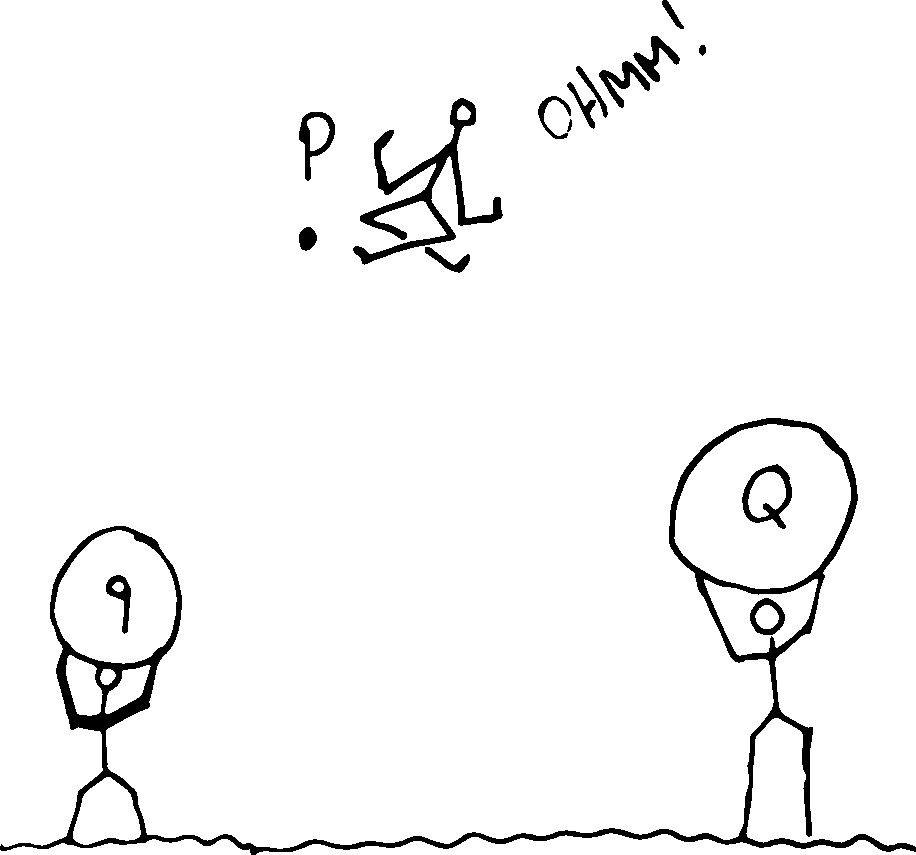
\includegraphics[scale=0.3]{figures/champ-deux-charges-1.pdf}
  \end{center}
\end{frame}


\begin{frame}{Tube à rayon cathodique}
  \begin{center}
    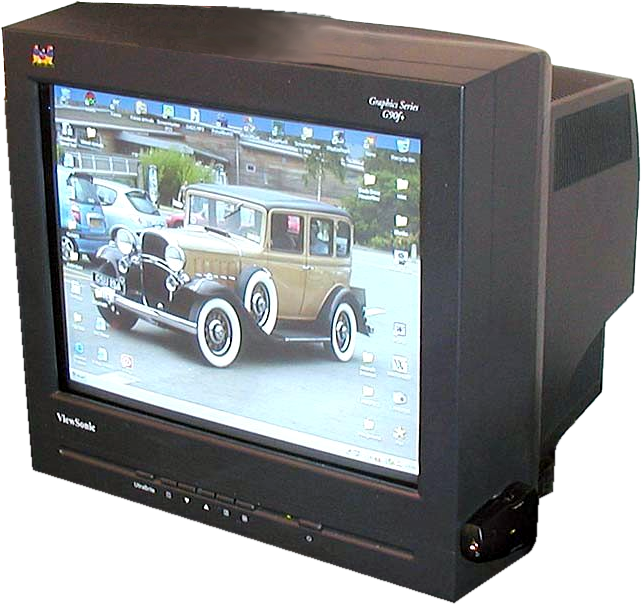
\includegraphics[scale=0.2]{figures/viewsonic-crt.png}
  \end{center}
\end{frame}


\begin{frame}{Tube à rayon cathodique}

  \begin{center}
  \begin{tikzpicture}[>=stealth, scale=0.8]
    \draw plot[smooth cycle] coordinates {(0, 1) (2, 1.5) (6, 3) (6, -3) (2, -1.5) (0, -1)};
    \draw[ultra thick] (0.8, 0.5) -- (2.5, 0.5);
    \draw[ultra thick] (0.8, -0.5) -- (2.5, -0.5);
    \foreach \x in {1.1, 1.5, 1.9, 2.3} {
      \node at (\x, 0.7) {$+$};
      \node at (\x, -0.7) {$-$};
    }
    \draw[thick, blue] plot[smooth] coordinates {(0, 0) (0.8, 0) (1.2, 0.02) (1.6, 0.04) (2, 0.08) (2.4, 0.16) (2.6, 0.2)} -- (6.4, 1.5);
    \draw[|<->|] (7, 3) -- node[fill=white] {$D$} (7, -3);
    \draw[|<->|] (0.8, -1.1) -- node[fill=white] {$l$} (2.5, -1.1);
    \draw[<->|] (2.5, -1.1) -- node[fill=white] {$L$} (6.4, -1.1);
  \end{tikzpicture}
  \end{center}

  Les dimensions du tube sont $l = \SI{2}{\centi\meter}$, $L =
  \SI{40}{\centi\meter}$ et $D = \SI{60}{\centi\meter}$.  Avant de passer entre
  les plaques du déflecteur, la vitesse des électrons est
  5\% de la vitesse de la lumière vers la droite.

  Déterminer la norme du champ électrique nécessaire pour que les électrons
  atteignent le haut de l'écran.

\end{frame}


\begin{frame}{Distribution de charge}
  Chaque disque et l'anneau ont tous la même charge $Q$.
  Classer les objets en ordre croissant de la grandeur du champ électrique au
  point $P$.

  \begin{center}
  \begin{tikzpicture}
    \matrix[row sep=1em, column sep=1em, ampersand replacement=\&] {
    \node at (0, -2.5) {(a)};
    \draw (0, 1.5) circle(1pt);
    \node[left] at (0, 1.5) {$P$};
    \draw (0,-2) -- (0,0);
    \draw[fill=black!10] (0,0) ellipse[x radius=1, y radius=0.5];
    \draw (0,0) -- (0,2);
    \draw (0,0) -- ++(-30:0.75);
    \node at (5:0.5) {$R$}; \&
    \node at (0, -2.5) {(b)};
    \draw (0, 1.5) circle(1pt);
    \node[left] at (0, 1.5) {$P$};
    \draw (0,-2) -- (0,0);
    \draw[fill=black!10] (0,0) ellipse[x radius=2, y radius=1];
    \draw (0,0) -- (0,2);
    \draw (0,0) -- ++(-30:1.5);
    \node at (-05:0.8) {$2R$}; \&
    \draw (0, 1.5) circle(1pt);
    \node[left] at (0, 1.5) {$P$};
    \node at (0, -2.5) {(c)};
    \draw (0,-2) -- (0,0);
    \draw[fill=black!10] (0,0) ellipse[x radius=2, y radius=1]; 
    \draw[fill=white] (0,0) ellipse[x radius=1, y radius=0.5];
    \draw (0,-0.5) -- (0,2);
    \draw (0,0) -- ++(-150:0.75);
    \node at (180:0.5) {$R$};
    \draw (0,0) -- ++(-30:1.5);
    \node at (-10:1.4) {$2R$};\\
    };
  \end{tikzpicture}
  \end{center}
\end{frame}
\end{document}
